\documentclass[margin=1cm,varwidth]{standalone}
\usepackage{amsfonts,amsmath,amssymb}
\usepackage[slovene]{babel}
\usepackage[utf8]{inputenc}
\usepackage[T1]{fontenc}
  
\usepackage{tikz, verbatim, subcaption}
\usepackage{pgfplots}
\usetikzlibrary{arrows.meta, calc, positioning, automata}

\newcommand{\subdiv}[3] {
\draw ($ 0.5*#2 + 0.5*#3 $) -- #1;
\draw ($ 0.5*#1 + 0.5*#3 $) -- #2;
\draw ($ 0.5*#1 + 0.5*#2 $) -- #3;
}

\captionsetup[subfigure]{labelformat=simple}
\renewcommand{\thesubfigure}{(\Alph{subfigure})}


\begin{document}

\begin{figure}
	\centering
% ####################   Simpleks S    ####################
	\begin{subfigure}[t]{0.5\linewidth}
		\centering
		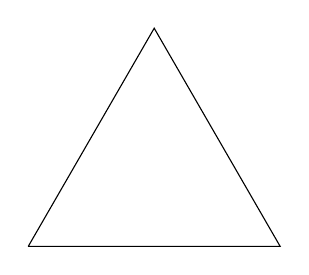
\begin{tikzpicture}[scale=0.4]
			\draw (0, 0) -- (8, 0) -- ($(4, {4*sqrt(3)})$) -- (0, 0);
		\end{tikzpicture}%
		\caption{Simpleks $S$.} \label{fig:simple}
	\end{subfigure}
	\vspace{0.5cm}
% ####################   Prva subdivizija    ####################
	\begin{subfigure}[t]{0.4\linewidth} 
		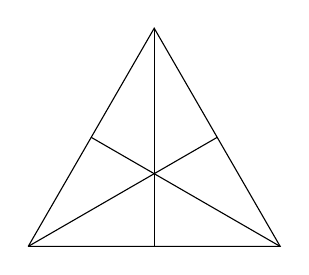
\begin{tikzpicture}[scale=0.4]
			\draw (0, 0) -- (8, 0) -- ($(4, {4*sqrt(3)})$) -- (0, 0);
			\subdiv{(0, 0)}{(8, 0)}{($(4, {4*sqrt(3)})$)}
		\end{tikzpicture}%
		\caption{Prva subdivizija.} \label{fig:triang}
	\end{subfigure}
	\quad
% ####################   Druga subdivizija    ####################
	\begin{subfigure}{0.5\linewidth}
		\centering
		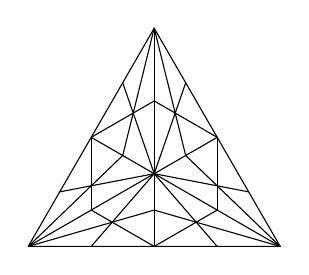
\begin{tikzpicture}[scale=0.4]
			\draw (0, 0) -- (8, 0) -- ($(4, {4*sqrt(3)})$) -- (0, 0);
			\subdiv{(0, 0)}{(8, 0)}{($(4, {4*sqrt(3)})$)}
			
			\subdiv{(0, 0)}{(4, 0)}{($(4, {4*sqrt(3)/3})$)}
			\subdiv{(0, 0)}{($(2, {2*sqrt(3)})$)}{($(4, {4*sqrt(3)/3})$)}
			\subdiv{($(4, {4*sqrt(3)})$)}{($(2, {2*sqrt(3)})$)}{($(4, {4*sqrt(3)/3})$)}
			\begin{scope}[xscale=-1,xshift=-8cm]
			\subdiv{(0, 0)}{(4, 0)}{($(4, {4*sqrt(3)/3})$)}
			\subdiv{(0, 0)}{($(2, {2*sqrt(3)})$)}{($(4, {4*sqrt(3)/3})$)}
			\subdiv{($(4, {4*sqrt(3)})$)}{($(2, {2*sqrt(3)})$)}{($(4, {4*sqrt(3)/3})$)}
			\end{scope}
		\end{tikzpicture}
		\caption{Druga subdivizija.} \label{fig:nitriang}  
	\end{subfigure}
	% ####################   Tretja subdivizija    ####################
	\begin{subfigure}{0.5\linewidth}
		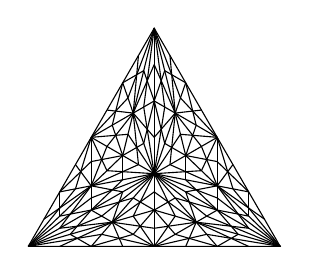
\begin{tikzpicture}[scale=0.4]
			\draw (0, 0) -- (8, 0) -- ($(4, {4*sqrt(3)})$) -- (0, 0);
			\subdiv{(0, 0)}{(8, 0)}{($(4, {4*sqrt(3)})$)}
			
			\subdiv{(0, 0)}{(4, 0)}{($(4, {4*sqrt(3)/3})$)}
			\subdiv{(0, 0)}{($(2, {2*sqrt(3)})$)}{($(4, {4*sqrt(3)/3})$)}
			\subdiv{($(4, {4*sqrt(3)})$)}{($(2, {2*sqrt(3)})$)}{($(4, {4*sqrt(3)/3})$)}
			
			\subdiv{(0, 0)}{(2, 0)}{($(8/3, {4*sqrt(3)/9})$)}
			\subdiv{(4, 0)}{(2, 0)}{($(8/3, {4*sqrt(3)/9})$)}
			\subdiv{(0, 0)}{(2, {2*sqrt(3)/3})}{($(8/3, {4*sqrt(3)/9})$)}
			\subdiv{(4, 0)}{(4, {2*sqrt(3)/3})}{($(8/3, {4*sqrt(3)/9})$)}
			\subdiv{($(4, {4*sqrt(3)/3})$)}{(2, {2*sqrt(3)/3})}{($(8/3, {4*sqrt(3)/9})$)}
			\subdiv{($(4, {4*sqrt(3)/3})$)}{(4, {2*sqrt(3)/3})}{($(8/3, {4*sqrt(3)/9})$)}
			
			\subdiv{($(4, {4*sqrt(3)/3})$)}{(2, {2*sqrt(3)/3})}{($(2, {10*sqrt(3)/9})$)}
			\subdiv{(0, 0)}{(2, {2*sqrt(3)/3})}{($(2, {10*sqrt(3)/9})$)}
			\subdiv{(0, 0)}{(1, {4*sqrt(3)/4})}{($(2, {10*sqrt(3)/9})$)}
			\subdiv{($(2, {2*sqrt(3)})$)}{(1, {4*sqrt(3)/4})}{($(2, {10*sqrt(3)/9})$)}
			\subdiv{($(2, {2*sqrt(3)})$)}{(3, {5*sqrt(3)/3})}{($(2, {10*sqrt(3)/9})$)}
			\subdiv{($(4, {4*sqrt(3)/3})$)}{(3, {5*sqrt(3)/3})}{($(2, {10*sqrt(3)/9})$)}
			
			\subdiv{($(2, {2*sqrt(3)})$)}{(3, {5*sqrt(3)/3})}{($(10/3, {22*sqrt(3)/9})$)}
			\subdiv{($(4, {4*sqrt(3)/3})$)}{(3, {5*sqrt(3)/3})}{($(10/3, {22*sqrt(3)/9})$)}
			\subdiv{($(2, {2*sqrt(3)})$)}{(3, {3*sqrt(3)})}{($(10/3, {22*sqrt(3)/9})$)}
			\subdiv{($(4, {4*sqrt(3)/3})$)}{(4, {8*sqrt(3)/3})}{($(10/3, {22*sqrt(3)/9})$)}
			\subdiv{($(4, {4*sqrt(3)})$)}{(3, {3*sqrt(3)})}{($(10/3, {22*sqrt(3)/9})$)}
			\subdiv{($(4, {4*sqrt(3)})$)}{(4, {8*sqrt(3)/3})}{($(10/3, {22*sqrt(3)/9})$)}
			\begin{scope}[xscale=-1,xshift=-8cm]
			\subdiv{(0, 0)}{(4, 0)}{($(4, {4*sqrt(3)/3})$)}
			\subdiv{(0, 0)}{($(2, {2*sqrt(3)})$)}{($(4, {4*sqrt(3)/3})$)}
			\subdiv{($(4, {4*sqrt(3)})$)}{($(2, {2*sqrt(3)})$)}{($(4, {4*sqrt(3)/3})$)}
			
			\subdiv{(0, 0)}{(2, 0)}{($(8/3, {4*sqrt(3)/9})$)}
			\subdiv{(4, 0)}{(2, 0)}{($(8/3, {4*sqrt(3)/9})$)}
			\subdiv{(0, 0)}{(2, {2*sqrt(3)/3})}{($(8/3, {4*sqrt(3)/9})$)}
			\subdiv{(4, 0)}{(4, {2*sqrt(3)/3})}{($(8/3, {4*sqrt(3)/9})$)}
			\subdiv{($(4, {4*sqrt(3)/3})$)}{(2, {2*sqrt(3)/3})}{($(8/3, {4*sqrt(3)/9})$)}
			\subdiv{($(4, {4*sqrt(3)/3})$)}{(4, {2*sqrt(3)/3})}{($(8/3, {4*sqrt(3)/9})$)}
			
			\subdiv{($(4, {4*sqrt(3)/3})$)}{(2, {2*sqrt(3)/3})}{($(2, {10*sqrt(3)/9})$)}
			\subdiv{(0, 0)}{(2, {2*sqrt(3)/3})}{($(2, {10*sqrt(3)/9})$)}
			\subdiv{(0, 0)}{(1, {4*sqrt(3)/4})}{($(2, {10*sqrt(3)/9})$)}
			\subdiv{($(2, {2*sqrt(3)})$)}{(1, {4*sqrt(3)/4})}{($(2, {10*sqrt(3)/9})$)}
			\subdiv{($(2, {2*sqrt(3)})$)}{(3, {5*sqrt(3)/3})}{($(2, {10*sqrt(3)/9})$)}
			\subdiv{($(4, {4*sqrt(3)/3})$)}{(3, {5*sqrt(3)/3})}{($(2, {10*sqrt(3)/9})$)}
			
			\subdiv{($(2, {2*sqrt(3)})$)}{(3, {5*sqrt(3)/3})}{($(10/3, {22*sqrt(3)/9})$)}
			\subdiv{($(4, {4*sqrt(3)/3})$)}{(3, {5*sqrt(3)/3})}{($(10/3, {22*sqrt(3)/9})$)}
			\subdiv{($(2, {2*sqrt(3)})$)}{(3, {3*sqrt(3)})}{($(10/3, {22*sqrt(3)/9})$)}
			\subdiv{($(4, {4*sqrt(3)/3})$)}{(4, {8*sqrt(3)/3})}{($(10/3, {22*sqrt(3)/9})$)}
			\subdiv{($(4, {4*sqrt(3)})$)}{(3, {3*sqrt(3)})}{($(10/3, {22*sqrt(3)/9})$)}
			\subdiv{($(4, {4*sqrt(3)})$)}{(4, {8*sqrt(3)/3})}{($(10/3, {22*sqrt(3)/9})$)}
			\end{scope}
		\end{tikzpicture}
		\caption{Tretja subdivizija.} \label{fig:nitriang}  
	\end{subfigure}
\caption{Slika prikazuje primer prve, druge in tretje subdivizije.}
\end{figure} 

\end{document}